%!TEX root = ../notas_de_clase.tex


\section{Anexos} 

\subsection{¿Qué hizo efectivamente Bayes y por qué?} 
   

Thomas Bayes fue uno de los primeros \emph{inconformistas anglicanos}.\footnote{ Este término se usa para denotar a los protestantes que no estaban de acuerdo con los métodos y la gobernanza eclesiástica establecida por la ``Iglesia de Inglaterra'' (The Church of England).} Su trabajo de 1763, titulado 
\begin{center}
\it
An Essay Towards Solving a Problem in the Doctrine of Chances
\end{center}
esbozó por primera vez el resultado que hoy conocemos como el Teorema de Bayes. Este trabajo fue terminado por el amigo y colega de Bayes, Richard Price (1723 – 1791), el cual  envió el artículo a la prestigiosa revista inglesa \emph{Philosophical Transactions of the Royal Society} (PTRS), donde fue publicado póstumamente. Este artículo consideraba el caso de \emph{invertir la distribución binomial}: en un experimento donde el resultado puede ser éxito  (con probabilidad $p$) o fracaso (con probabilidad $1-p$), el objetivo es encontrar la distribución del parámetro $p$ dado que se han observado $q$ éxitos luego de $n$ experimentos. Para resolver este caso particular, Bayes descubrió que efectivamente la distribución posterior es proporcional a la verosimilitud. Sin embargo, a pesar de que Price completara el trabajo de Bayes  luego de la repentina muerte de éste último, este trascendental descubrimiento quedó momentáneamente en el olvido. Fue finalmente Laplace quien en 1774 publicó la relación entre las distribuciones  prior y posterior como la conocemos hoy, sin dejar de reconocer el trabajo de Bayes. En efecto, en su \emph{Essai Philosophique dur les Probabilites} (1814), Laplace menciona que Bayes ya había llegado al mismo resultado de forma ``refinada y muy ingeniosa, aunque un poco confusa''.\\

Existen dudas sobre la autoría de Bayes del artículo en cuestión y cuánto de éste efectivamente venía de las propias notas no publicadas de Bayes, y cuánto de la edición y cálculos de R. Price \cite{bellhouse_2004}. En efecto, al año siguiente del artículo original, Price publicó en 1764 otro artículo en PTRS llamado \emph{A Demonstration of the Second Rule in the Essay toward the Solution of a Problem in the Doctrine of Chances}, esta vez de su propia autoría. Tanto Bayes como Price estaban muy lejos de ser  matemáticos prolíficos de su época, de hecho, las publicaciones de ambos no están particularmente ligadas a las matemáticas sino que son de índole religiosa---por mucho que sus contribuciones hayan sido suficientemente  conceptuales y generales para ser consideradas como avances en ambos campos. Una posibilidad para entender las motivaciones de Bayes (y Price) para el desarrollo de los artículos mencionados, pueden encontrarse en el artículo \cite{stigler2013} el cual postula que el verdadero título del artículo de Bayes aparentemente es: 
\begin{center}
\it
A Method of Calculating the Exact Probability of All Conclusions founded on Induction.
\end{center}
Este título, según explica \cite{stigler2013}, pudo haber sido perdido en la edición del artículo o probablemente el propio editor de PTRS lo modificó por encontrarlo un tanto \emph{atrevido}.  Si este fuese efectivamente el título, y no el menos informativo título original, se entiende que el artículo tiene por objetivo caracterizar  el problema más general de \emph{inducción}. Esto tiene un sentido particular dado el contexto filosófico y religioso en ese entonces, pues pocos años antes la obra de Hume `Of Miracles' (1748) presentaba un argumento probabilístico para desestimar los milagros (como la resurrección). En  pocas  palabras, Hume postulaba que la considerable \emph{improbabilidad} de un milagro sobrepasaba ampliamente la \emph{probabilidad}  de  que el milagro fuese incorrectamente  documentado. Este ensayo de Hume fue ampliamente leído, discutido y---evidentemente---atacado, en particular, tanto Bayes como Price, ambos inconformistas anglicanos, consideraron  el ensayo de Hume como una agresión. Consecuentemente, Bayes consideró responder al argumento de  Hume mediante la aplicación de probabilidades al problema de inducción, lo cual es confirmado por las notas no publicadas de Bayes con fecha anterior al 31 de diciembre de 1749 \cite{bellhouse_2004}, las que eventualmente llegaron al famoso artículo de 1763. Sin embargo, el trabajo de Bayes no estaba completo, en particular, no contaba una satisfactoria aproximación de la distribución posterior en el ejemplo de la inversión de la distribución binomial mencionado anteriormente. En este sentido, la motivación de Price para terminar este trabajo no era únicamente concluir el trabajo póstumo de su amigo, sino que también desarrollar un respuesta eficaz contra el argumento de Hume. En efecto, luego de una serie de  trabajos relacionados, fue  finalmente en 1767 que Price logró publicar su disertación \emph{On the Importance of Christianity, its Evidences, and the Objections which have been made to it}, donde hace una crítica directa a “Of miracles”. Básicamente, Price sentencia que Hume habría subestimado el impacto que una (gran) cantidad de observadores \textbf{independientes} reportando la existencia del milagro puede tener. En dicho caso, el Teorema de Bayes mostraba que la multiplicación de evidencia, la cual puede ser falible de forma individual, podría sobrepasar la improbabilidad de un evento (el milagro) y establecerlo como verdad (o en realidad muy probable). \\

Existen varias razones atribuibles a que el trabajo de Bayes haya sido ignorado parcialmente hasta Laplace, e.g., la incompletitud del trabajo del propio Bayes, el rol incierto que tuvo Price en el desarrollo de éste, y el nombre poco elocuente del artículo que probablemente desvió atención al trabajo. Todo esto nos hace cuestionarnos si es correcto referimos a este trascendental Teorema en honor al Rev.~Thomas Bayes, el cual lanzó el primer atisbo de este resultado y no a Laplace, el cual fue el primero en enunciar la forma general para la relación entre prior, posterior y modelo en la forma que hoy conocemos y usamos. 

\subsection{Álgebra lineal}

\subsubsection{Cálculo matricial}

Para dos vectores $\x\in\R^n$, $\y\in\R^m$, el operador $\frac{\partial \y}{\partial \x}$ puede ser definido como una matriz de dos formas distintas dependiendo del orden en el que se completen las entradas de la matriz:

\begin{itemize}
	\item Notación jacobiana (numerator-layout): la matriz se completa de acuerdo a $\y$ y $\x^\top $, es decir:
	\begin{equation*}
		\left(\frac{\partial \y}{\partial \x}\right)_{ij} = \frac{\partial y_i}{\partial x_j} \implies \frac{\partial \y}{\partial \x}\in \mathcal{M}_{mn}(\R)
	\end{equation*}
	
	\item Notación hessiana (denominator-layour): la matriz se completa de acuerdo a $x$ e $y^\top $, es decir:
	\begin{equation*}
		\left(\frac{\partial \y}{\partial \x}\right)_{ij} = \frac{\partial y_j}{\partial x_i} \implies \frac{\partial \y}{\partial \x}\in \mathcal{M}_{nm}(\R)
	\end{equation*}
	
\end{itemize}


La notación estandar corresponde a la notación jacobiana y es la que se sigue a lo largo del apunte. Bajo esta notación, la derivada de un campo vectorial (gradiente) corresponde a un vector vertical cuyas componentes son las derivadas de las componentes del campo.\\

Sean $\x$, $\bf{u}=\bf{u}(\x)$, $\bf{v}=\bf{v}(\x)$ y $\bf{a}$ vectores, $\bf{g}$ campo vectorial y $A$ matriz de dimensiones apropiadas. Bajo la convención de la notación jacobiana, se tienen las siguientes fórmulas de derivación:

\begin{itemize}

	\item Transformación lineal:
	\begin{equation}
		\frac{\partial (A\x)}{\partial \x}=A \implies \begin{cases}
		\frac{\partial \x}{\partial \x} = I\\
			\frac{\partial (\x^\top A)}{\partial \x} = A^\top  \text{ ya que } \frac{\partial \bf{u}^\top }{\partial \x} = \left( \frac{\partial \bf{u}}{\partial \x}\right)^\top
		\end{cases}
	\end{equation}
	
	\item Producto punto:
	\begin{equation}
		\frac{\partial (\bf{u}\cdot \bf{v})}{\partial \x} = \bf{u}^\top \frac{\partial \bf{v}}{\partial \x} + \bf{v}^\top  \frac{\partial \bf{u}}{\partial \x} \implies \begin{cases}
 	\frac{\partial (\bf{a}\cdot \x)}{\partial \x} = \bf{a}^\top\\
 	\frac{\partial (\x\cdot \x)}{\partial \x} = \frac{\partial \norm{\x}^2}{\partial \x} = 2\x^\top 
 \end{cases}
	\end{equation}
	
	\item Forma cuadrática:
	\begin{equation}
		\frac{\partial (\textbf{u}^\top A \textbf{v})}{\partial \x} = \textbf{u}^\top A \frac{\partial \bf{v}}{\partial \x} + \textbf{v}^\top A^\top  \frac{\partial \bf{u}}{\partial \x} \implies \begin{cases}
 	\frac{\partial (\x^\top A\x)}{\partial \x} = \x^\top(A+A^\top)=2\x^\top A\text{ si $A$ es simétrica}.\\
 	\frac{\partial^2 (\x^\top A\x)}{\partial \x \partial \x^\top} = A + A^\top =2A\text{ si $A$ es simétrica}.
 \end{cases}
	\end{equation}
	
	\item Regla de la cadena:
	\begin{equation}
		\frac{\partial (\bf{g}(\bf{u}))}{\partial \x} = \frac{\partial \bf{g}(\bf{u})}{\partial \bf{u}} \frac{\partial \bf{u}}{\partial \x}
	\end{equation}

\end{itemize}

Por otra parte, si $x$ es una variable escalar e $Y\in\mathcal{M}_{mn}(\R)$ es una matriz dependiente de $x$, se define $\frac{\partial Y}{\partial x}$ como la matriz $Y$ con el operador derivada aplicado a cada entrada, es decir:

	\begin{equation*}
		\left(\frac{\partial Y}{\partial x}\right)_{ij} = \frac{\partial Y_{ij}}{\partial x} \implies \frac{\partial Y}{\partial x}\in \mathcal{M}_{mn}(\R)
	\end{equation*}

Bajo esta definición, si $U,V$ son matrices dependientes de $x$ de dimensiones apropiadas, entonces se tienen las siguientes reglas de derivación:

\begin{itemize}
	\item Regla del producto:
	\begin{equation}
		\frac{\partial (UV)}{\partial x} = U \frac{\partial V}{\partial x} + \frac{\partial U}{\partial x}V
	\end{equation}
	
	\item Inversa (para $U$ invertible):
	\begin{equation}
		\frac{\partial U^{-1}}{\partial x} = -U^{-1} \frac{\partial U}{\partial x}-U^{-1}
	\end{equation}
\end{itemize}

Por último, sea $X\in\mathcal{M}_{mn}(\R)$ una matriz e $y$ un escalar dependiente de $X$. Bajo la notación jacobiana, se tiene la siguiente definición:

\begin{equation*}
		\left(\frac{\partial y}{\partial X}\right)_{ij} = \frac{\partial y}{\partial X_{ji}} \implies \frac{\partial y}{\partial X}\in \mathcal{M}_{nm}(\R)
	\end{equation*}
	
Sean $u=u(X),v=v(X)$ escalares, $g$ función real, $H$ función matricial y $A,B$ matrices. Se tienen las siguientes reglas de derivación:

\begin{itemize}
	\item Producto de escalares:
	\begin{equation}
		\frac{\partial uv}{\partial X} = u\frac{\partial v}{\partial X} + v\frac{\partial U}{\partial X}
	\end{equation}
	
	\item Regla de la cadena:
	\begin{equation}
		\frac{\partial g(u)}{\partial X} = \frac{\partial g(u)}{\partial u} \frac{\partial u}{\partial X}
	\end{equation}
	
	\item Operador traza:
	\begin{equation}
		\frac{\partial \text{Tr}(H(X))}{\partial X} = H'(X),	\text{ en particular } \begin{cases}
			\frac{\partial \text{Tr}(AX)}{\partial X} = A\\
			\frac{\partial \text{Tr}(x^\top A X)}{\partial X} = X^\top(A+A^\top)\\
			\frac{\partial \text{Tr}(AXB)}{\partial X} = BA\\
			\frac{\partial \text{Tr}(X^n)}{\partial X} = nX^{n-1}
		\end{cases}
		\end{equation}
\end{itemize}

Sean X matriz invertible, entonces 
\begin{equation}
\frac{\partial |X|}{\partial X} = |X|X^{-T} 
\end{equation}
\begin{equation}
\frac{\partial x^\top X^{-1} x }{\partial X} = -X^{-\top}xx^\top X^{-\top}
\end{equation}

\subsubsection{Rango e inversa de Moore-Penrose}

\begin{definition}[rango]
	Para una matriz $M\in\mathcal{M}_{mn}(\R)$ se define su rango como el número máximo de filas (equivalentemente, columnas) linealmente independientes que tiene la matriz.
\end{definition}

Por lo tanto, una matriz cuadrada es invertible si y solo si tiene rango máximo (todas sus filas y columnas son l.i.). De este modo, se tiene la siguiente propiedad:

\begin{lemma}
	Sea $A\in\mathcal{M}_{mn}(\R)$ entonces $A^\top A \in\mathcal{M}_{nn}(\R)$ es invertible si y solo si $A$ tiene todas sus columnas l.i.
\end{lemma}

En efecto, dado que $r(M_1M_2)\leq\min\{r(M_1),r(M_2)\}$ entonces, $A^\top A \in\mathcal{M}_{nn}(\R)$ es invertible si y solo si $r(A^\top A)=n\iff r(A^\top )=r(A)=n$, por lo que $A$ tiene $n$ columnas (y filas) l.i.\\

Debido a esto es que para poder utilizar la fórmula de regresión lineal mediante MC o MCR necesariamente $\hat{X} \in\mathcal{M}_{N,M+1}(\R)$ debe ser de rango $M+1$ (máximo por columnas), lo cual es equivalente a pedir que las $M+1$ observaciones sean l.i.\\

\begin{definition}[pseudoinversa de Moore-Penrose] Sea $A\in\mathcal{M}_{mn}(\R)$. Otra matriz $A^+\in\mathcal{M}_{nm}(\R)$ se dice que es la pseudoinversa de $A$ si:

\begin{itemize}
	\item (inversa débil) $AA^+A=A$ y $A^+AA^+=A^+$
	\item (simetría) $(AA^+)^\top  = AA^+$ Y $(A^+A)^\top  = A^+A$
\end{itemize}
	
\end{definition}

Se puede probar que la pseudoinversa siempre existe. Además, por el lema anterior se tiene que si $A$ es de rango completo, entonces la pseudoinversa tiene forma cerrada:

\begin{itemize}
	\item $A$ tiene columnas l.i. $\implies A^+=(A^\top A)^{-1}A^\top $ y es inversa por izquierda: $A^+A=I$.
	\item $A$ tiene filas l.i. $\implies A^+=A^\top (AA^\top )^{-1}$ y es inversa por derecha: $AA^+=I$.
\end{itemize}

De este modo, en la regresión por MC, la solución $\theta=\hat{X}^+Y$ puede ser interpretada como el proceso de despejar $\theta$ en la hipótesis $Y=X\theta$.

\subsubsection{Fórmula de Woodburry}

Esta fórmula permite descomponer la inversa de una suma particular de matrices.

\begin{theorem}[Fórmula de Woodburry]
	Para matrices de dimensiones adecuadas, se tiene la siguiente fórmula de inversión:
	
	\begin{equation}
		(A+UCV)^{-1} = A^{-1} - A^{-1}U(C^{-1}+VA^{-1}U)^{-1}VA^{-1}
	\end{equation}
\end{theorem}

Esta descomposición puede ser demostrada directamente probando que al multiplicar $A+UCV$ por la igualdad de la derecha se obtiene la identidad.

\subsection{Optimización}
\subsubsection{Teorema de Karush-Khun-Tucker}

Sean $f:E\subset\R^n\to\R$, $g:\R^n \to \R^m$ y $h:\R^n \to \R^p$ funciones diferenciables. Un problema de optimización con estructura de Karush-Kuhn-Tucker viene dado por:
\begin{equation}
	\begin{aligned}
		(P) & \min_{s.a} f(x)\\
		& g(x) \leq 0\\
		& h(x) = 0\\
		& x\in E
	\end{aligned}
\end{equation}
	

Donde $g(x) \leq 0\iff g_i(x)\leq 0,\forall i\in\{1,\ldots,m\}$.\\

Sea $x_0$ un punto factible de $(P)$ tal que $\left\{\{\nabla g_i(x_0)\}_{i=1}^m,\{\nabla h_i(x_0)\}_{i=1}^p\right\}$ es linealmente independiente. Si $x_0$ es solución de $(P)$, entonces existen $\mu\in\R^m$ y $\lambda\in\R^p$ tal que

\begin{equation}
	\begin{aligned}
		f(x) + \langle\lambda,g(x_0)\rangle + \langle\mu,h(x_0)\rangle &=0\\
		 u_i g_i(x_0) &= 0\\
		 u_i &\geq 0\\
	\end{aligned}
\end{equation}

\subsubsection{Método del gradiente clásico}

El método del gradiente es un método numérico iterativo que busca aproximar la solución del problema irrestricto

\begin{equation}
	\text{(P)} \min_{x\in \R^n} f(x)
\end{equation}

Donde las iteraciones son de la forma $x_{k+1} = x_k + \beta_k d_k$, con $d_k$ una dirección de descenso y $\beta_k$ la magnitud del desplazamiento (paso). El método del gradiente considera $d_k$ como la dirección de máximo descenso:

\begin{equation}
	d_k = \argmin_{\norm{d} = 1} \langle\nabla f(x_k),d\rangle \implies d_k = \frac{-\nabla f(x_k)}{\norm{\nabla f(x_k)}}
\end{equation}

Ya que el producto interno es máximo cuando los dos vectores son paralelos. Por otra parte, para $\beta_k$ se considerará el desplazamiento óptimo, el cual está dado por un problema de optimización unidimiensional:

\begin{equation}
	\beta_k = \argmin_{\beta\geq 0} f(x_k + \beta d_k) 
\end{equation}

De este modo, se tendrá un algoritmo iterativo que genera secuencias decrecientes en el valor de la función: $f(x_n)\geq f(x_m)$ para $m\geq n$.\\

Bajo ciertas condiciones sobre $f$ (convexidad y gradiente lipschitz) y elecciones particulares de $\beta_k$, se puede probar que el algoritmo converge a un mínimo global. \\

\begin{figure}[h]
  \centering
  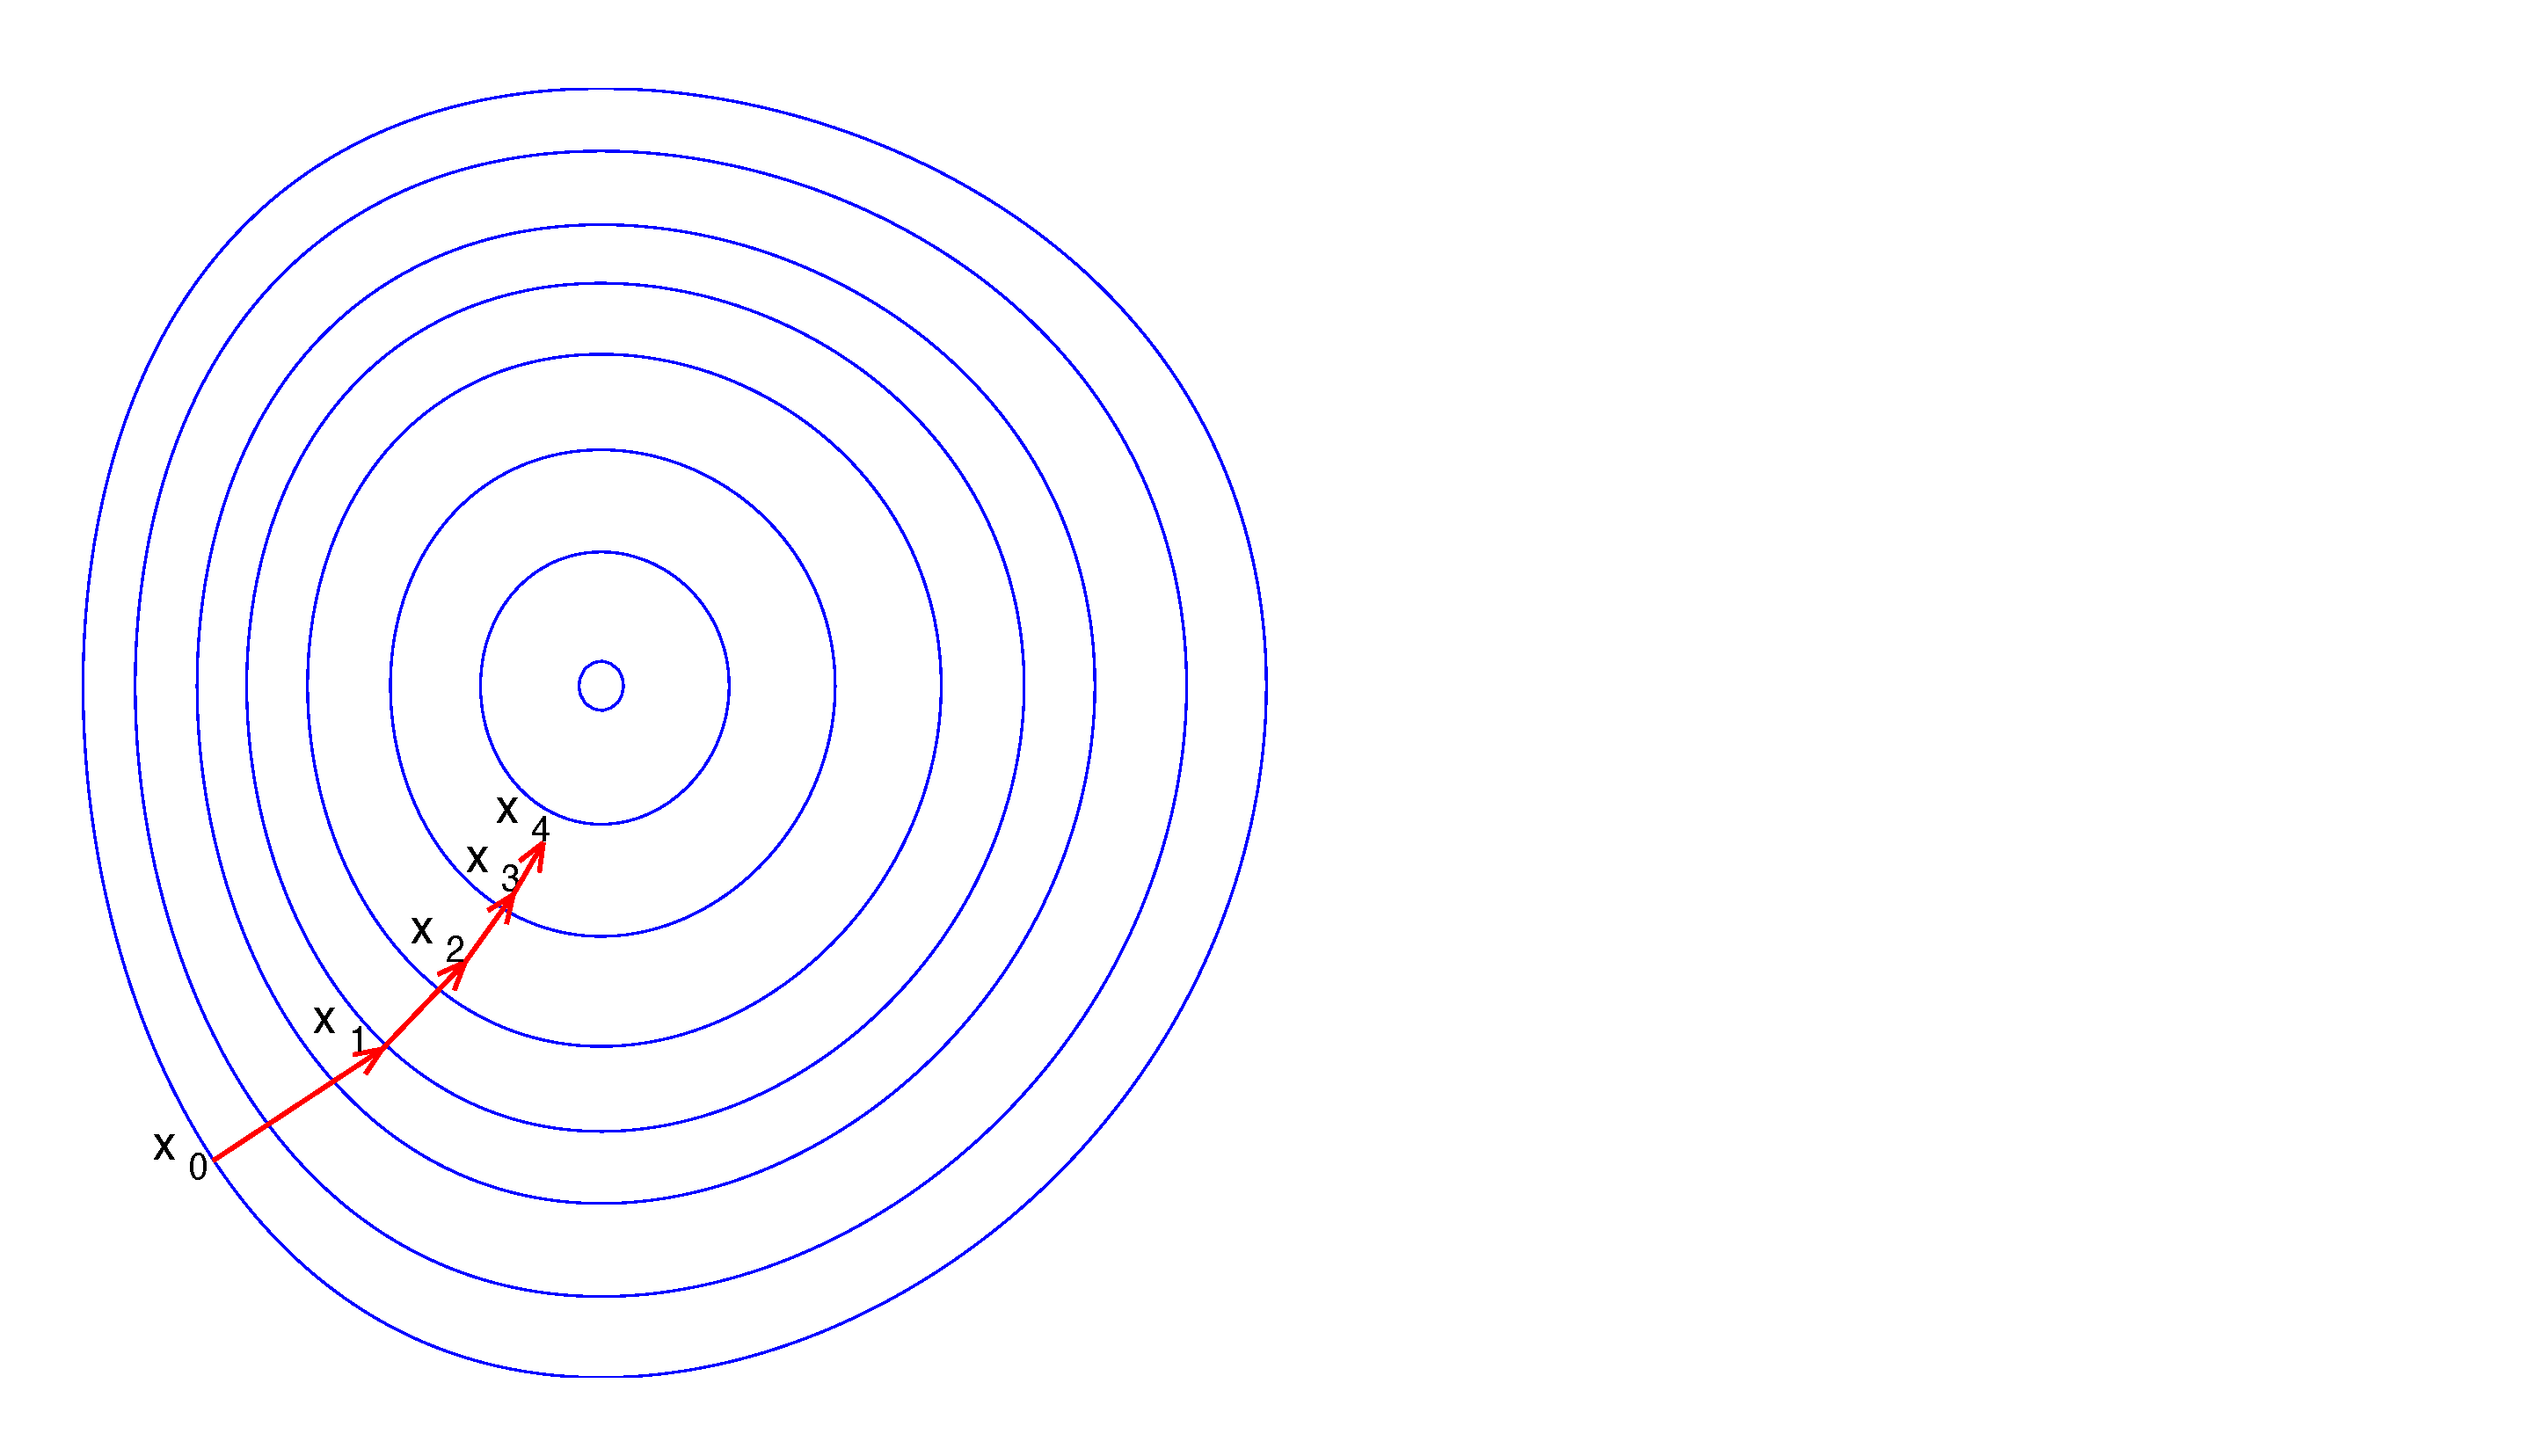
\includegraphics[width=12cm, height=8cm]{img/anexos_gd.pdf}
  \caption{Iteraciones del método del gradiente para una función de ejemplo.}
\end{figure}

El algoritmo se detiene cuando se alcanza una cierta tolerancia de error, la cual es obtenida cuando la norma del gradiente es suficientemente pequeña, lo que indica que no habrá mucha variación entre la iteración actual y la siguiente.

\subsubsection{Dualidad lagrangiana}

Sean $f:E\subset\R^n\to\R$, $g:\R^n \to \R^m$ y $h:\R^n \to \R^p$ funciones diferenciables y $(P)$ un problema de optimización con estructura de Karush-Kuhn-Tucker:
\begin{equation}
	\begin{aligned}
		(P) & \min_{s.a} f(x)\\
		& g(x) \leq 0\\
		& h(x) = 0\\
		& x\in E
	\end{aligned}
\end{equation}
	

El lagrangiano de $(P)$ corresponde a $L(x,\lambda,\mu) := f(x) + \langle\lambda,g(x)\rangle + \langle\mu,h(x)\rangle$, donde $\lambda$ y $\mu$ se denominan multiplicadores de Lagrange o variables duales. Se define la función lagrangiana dual como:

\begin{equation}
	\theta(\lambda,\mu):=\inf_{x\in E} L(x,\lambda,\mu)
\end{equation} 

De este modo, se tiene el problema lagrangiano dual:

\begin{equation}
	(D) \max_{\lambda\geq 0} \theta(\lambda,\mu)
\end{equation}

\begin{theorem}[dualidad fuerte]
	Sea $E\subset\R$ convexo no vacío, $f,g$ convexas y $h$ afín (es decir, de la forma $h(x) = Ax+b$). Supóngase que:

\begin{itemize}
	\item $\exists x\in E:g(x)<0, h(x)=0$.
	\item $0\in \text{int}(\text{Im}(h))$.
\end{itemize}

Entonces, $(P)$ y $(D)$ tienen el mismo valor óptimo límite (como ínfimo y supremo) y si dicho valor es finito, entonces el supremo es alcanzado en el problema dual. Además, si en $(P)$ el ínfimo es alcanzado en $\hat{x}\in E$ entonces $\langle \mu,g(\hat{x})\rangle=0$.
\end{theorem}
	
En el caso de un problema convexo con restricciones de desigualdad diferenciables, el ínfimo del lagrangiano es alcanzado donde se anula su gradiente, de este modo, la función lagrangiana dual tiene forma explícita y se tiene que:

\begin{equation}
	\begin{aligned}
		(P) & \min_{s.a} f(x)\\
		& g(x) \leq 0\\
	\end{aligned} \implies
	\begin{aligned}
		(D) & \max_{\lambda\geq 0} L(x,\lambda)= f(x) + \langle\lambda,g(x)\rangle\\
		& \nabla_x L(x,\lambda) = \nabla f(x) + \langle\lambda,\nabla g(x)\rangle = 0\\
	\end{aligned}
\end{equation}


\begin{theorem}[holgura complementaria]
	Bajo las hipótesis de dualidad fuerte, si el ínfimo de $(P)$ es alcanzado en $\hat{x}$ y el supremo de $(D)$ es alcanzado en $(\hat{\lambda},\hat{\mu})$ entonces $\lambda_i f_i(\hat{x})=0, \forall i\in\{1,\ldots,m\}$.
\end{theorem}
